\section{The Solenoid and the Steel Return Yoke}
\label{sec:solenoid}

The Compact Muon \emph{Solenoid} sports one of the world's most energetic solenoids, which is absolutely indispensable to the success of CMS.
It is a huge 6 meter-tall and 13 meter-long cylindrical magnet that generates a uniform magnetic field parallel to the beam line.
% the direction in which the protons collide, which we call the z direction.
When charged particles travel through this volume a Lorentz force is applied to them,
thereby separating out the particle tracks as they fly away from the IP.
% As the charged particles bend out and away from the beam pipe, they pass through the silicon tracking system, which has excellent resolution ""
% Imagine CMS as a giant camera that takes a picture every few ns of the outgoing particles. 
An enormous current of 18,000 A travels through superconducting Nb-Ti coils to produce the uniform 3.8 T magnetic field inside the volume of the solenoid (approximately 360 m$^3$)
 (Fig.~\ref{fig:cms_magnetic_field}).
%%%%%%%%%%%%%%%%%%%%
\begin{figure}[pbth]
\centering
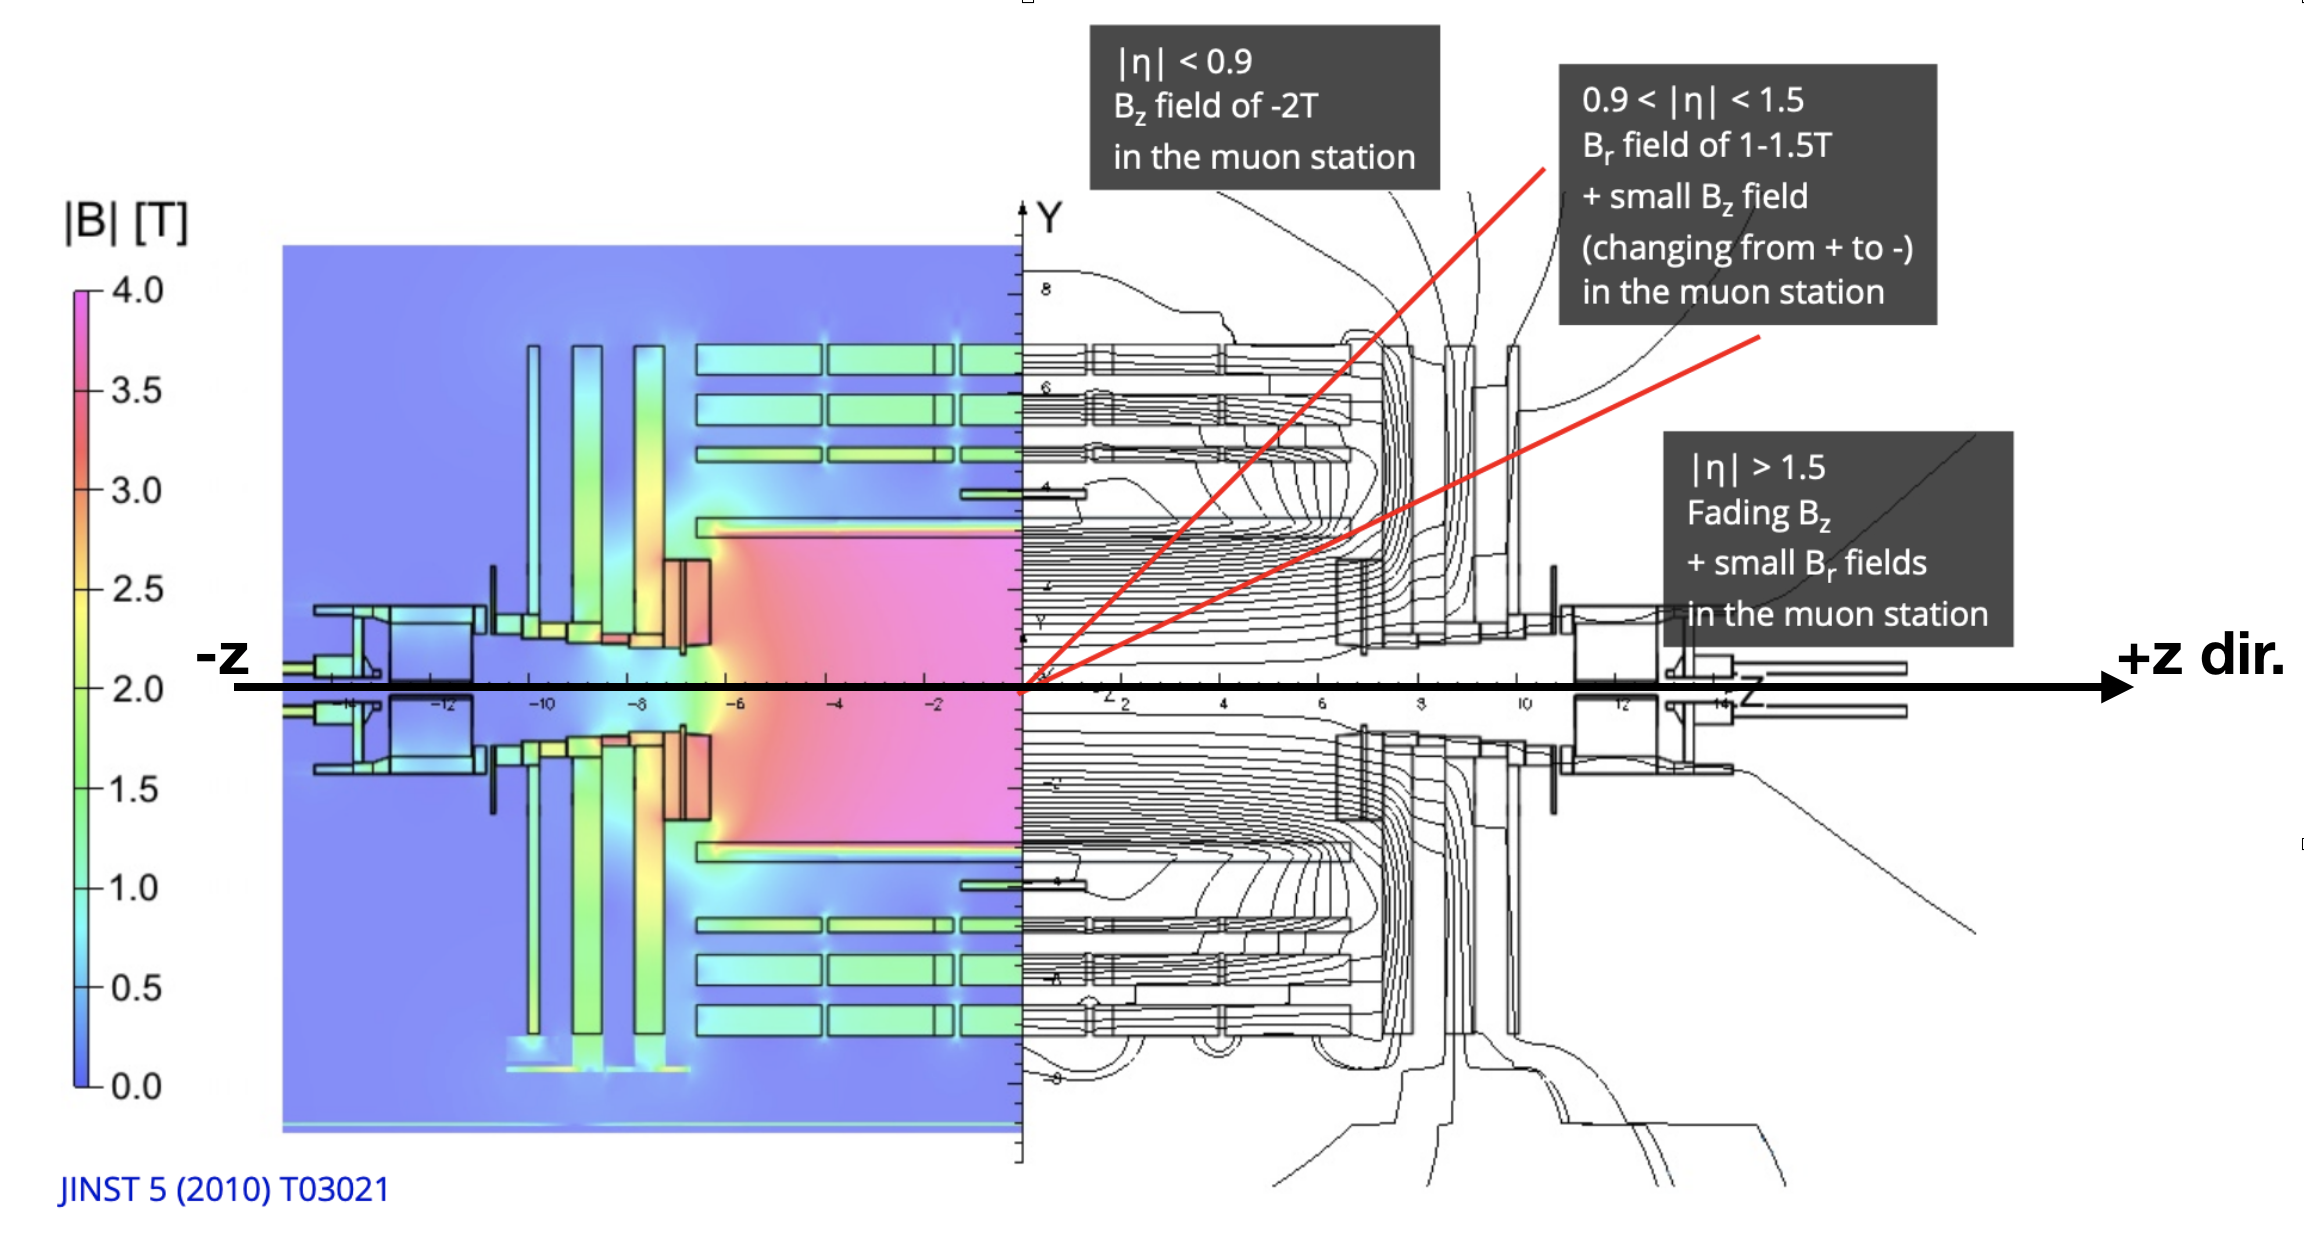
\includegraphics[width=15cm,height=15cm,keepaspectratio]{Figures/CMS_longitudinal_view_magnetic_field.png}
    \caption{
    A longitudinal cross section of CMS showing the values of the magnetic field over the volume of CMS and various field lines. 
    The magnetic field reaches its maximum of 3.8 T in the center of the detector.}
    \label{fig:cms_magnetic_field}
\end{figure}
%%%%%%%%%%%%%%%%%%%%
This magnetic field is 100,000 times stronger than the Earth's magnetic field.
A massive 2.7 GJ of energy is stored in the magnetic field of CMS. 
This is about the same amount of energy found in an Airbus A320 in flight!

{\bf Steel Return Yoke:} 
Most of the mass of CMS comes from the steel return yoke which helps to redirect the powerful magnetic field back on itself. 
The yoke system constitutes 12,500 tonnes, which is 89\% of CMS's total mass.
